\documentclass{article}

\usepackage[a4paper, total={6.2in, 8in}]{geometry}
\usepackage{pgfplots}
\pgfplotsset{compat=1.18}
\usepackage{graphicx}
\usepackage{array}
\usepackage{hhline}
\usepackage{subcaption}
\usepackage{lipsum}
\usepackage{blindtext}
\usepackage{titlesec}

\setlength\parindent{0pt}

\title{\LARGE\bfseries An Assessment of the Potential Behaviours of Self-Driving Cars}
\author{
     \\
     \\
\textbf{By Luke Guppy} \\
    \\
    \\
    \\
    \\
\centerline{\rule{10cm}{0.4pt}}\\
    \\
    \\
\textbf{University of Warwick} \\
\\
Department of Computer Science \\
\\
Supervisor: Andrew Hague \\
\\
Year of Study: $3^{rd}$ \\
\\
2024 \\
    \\
\centerline{\rule{10cm}{0.4pt}}
}
\date{}

\begin{document}
\maketitle
\newpage

\section*{Abstract}
This project aims to explore an implementation of curriculum learning to train self-driving cars within a simulation environment. The aim is to equip the car agent with the ability to navigate an environment while adhering to traffic rules and avoiding collisions. Through the use of Unity simulation and the ML-Agents package, the project focuses on developing an agent capable of path following, lane centering, responding appropriately to traffic lights, and environmental cars.\\

Throughout the development process, multiple stages of reward systems were devised and iteratively refined to incentivise desired behaviours, ultimately culminating in the creation of a successful framework and incremental introduction of the named behaviours. The resulting agent demonstrates proficient path following capabilities, effectively negotiating complex scenarios while following traffic regulations.\\

This project contributes to the advancement of autonomous vehicle technology by providing insights into the effectiveness of curriculum learning methodologies for training self-driving car agents. The modular nature of the simulation allows for flexible experimentation and evaluation of various training strategies. It also gives a strong insight as to how a reward system can be developed to iteratively implement new behaviours while also giving an understanding of the limitations of the Deep-Reinforcement Leaning system applied.

\noindent\hrulefill \\

Self-driving cars, Reinforcement learning, Autonomous agents, Simulation environments, Curriculum learning, Traffic simulation, Agent-based modeling, Reward optimisation

\newpage

\tableofcontents
\newpage


\section{Introduction to the Project}

\subsection{Refined Problem Statement and Addressed Gap}
In the world of deep-reinforcement learning, specifically in the field of autonomous cars, a gap exists in research of how to effectively develop a comprehensive reward system that allows a cumulative approach to implementing driving behaviours by autonomous agents. While existing research has made significant strides in designing reward systems tailored to specific functionalities, there remains a notable gap in the literature concerning the creation of a cohesive framework for integrating various behaviours and facilitating agent learning in a systematic manner. Although the field of autonomous driving is one of the largest growing industries in the world ``there are a few successful commercial applications, there is very little literature or large-scale public datasets available" \cite{Deep-learning-for-AI-driving}. This is the incentive which necessitates more research into how DRL can be applied in these situations to implement driving behaviours. \\

This project seeks to address this gap by adopting a novel approach that leverages curriculum learning principles to train autonomous agents within a simulated environment. The refined problem statement centers on the design and implementation of a holistic reward system capable of accumulating a range of driving behaviours, including lane navigation, traffic light interactions, obstacle avoidance, and path following. \\

Unlike traditional approaches that focus on isolated features and corresponding reward mechanisms, this project aims to establish a structured methodology for accumulating rewards and incrementally building up the capabilities of autonomous agents. By adopting a curriculum learning framework, the project aims to provide a scaffolded for deep-reinforcement learning, enabling agents to progressively acquire and master complex driving behaviors over time.\\

Through this innovative approach, the project not only aims to contribute to advancements in autonomous driving technology but also to bridge the gap between theoretical research and practical implementation. By developing a robust reward system structure and leveraging curriculum learning techniques, the project seeks to lay the foundation for the creation of adaptable and resilient autonomous agents capable of seamlessly integrating new behaviors and functionalities as they evolve.

\subsection{Motivation}
The motivation behind this project is rooted in the transformative potential of self-driving cars, which stand at the forefront of modern innovation in all aspects of technological advancements. With the promise of enhanced safety, efficiency, and accessibility, autonomous vehicles represent a shift in the way we perceive and interact with transportation systems \cite{mckinsey_autonomous_vehicles}. As the automotive industry continues to make strides towards the widespread adoption of autonomous technologies.\\

A key driving force behind this project is the rapid progression and advancements witnessed in the field of deep reinforcement learning (DRL). Building upon the foundations of traditional reinforcement learning, DRL has emerged as a powerful paradigm for training autonomous agents to make complex decisions and navigate complex environments. The integration of deep neural networks with reinforcement learning algorithms has unlocked new possibilities for training agents to exhibit human-like behaviours and adaptability \cite{robust_deep_learning}.\\

The field of artificial intelligence (AI) and DRL has provided a unique opportunity to overcome the inherent dangers posed by current road environments, characterised by diverse and unpredictable traffic scenarios, road conditions, and human behaviours. The prevalence of accidents and road-related fatalities underscores the need for an understanding of how to develop robust and reliable autonomous driving systems that can navigate safely and effectively \cite{junction_driving}. By leveraging advancements in reinforcement learning and curriculum learning methodologies, this project aims to address these challenges and provide an understanding in how to develop such systems not only in the field of autonomous driving but for any DRL agent.\\

The field of curriculum learning offers a promising avenue for training autonomous agents in a structured and systematic manner. By breaking down complex tasks into manageable sub-tasks and gradually increasing the difficulty level, curriculum learning enables agents to learn progressively and adapt to increasingly complex environments \cite{automatic_curriculum}. This project draws inspiration from the principles of curriculum learning to design a structured framework for training autonomous agents in a manner that imitates human and animal learning behaviours \cite{human_curriculum_learning}. This learning methodology allows for better adaptability and progression when learning where previous learning methods have struggled to implement complex behaviours. \\

Through the convergence of advancements in self-driving technology, deep reinforcement learning, and curriculum learning methodologies, this project seeks to contribute to the ongoing evolution of autonomous driving systems, driving innovation and progress towards safer, more efficient road systems.

\subsection{Objectives}
\begin{itemize}
    \item \textbf{Develop a Realistic Simulation Environment:} Create a Unity-based simulation environment that abstracts real-world driving scenarios, focusing on essential features while omitting minor details.
    
    \item \textbf{Design and Implement Learning Agents:} Develop a reinforcement learning agent, ensuring it can navigate the simulation environment effectively.
    
    \item \textbf{Conduct In-Depth Research:} Carry out comprehensive research on AI-driven cars, traffic dynamics, and human behaviour to inform the development of the simulation and learning agent.
    
    \item \textbf{Training and Performance Analysis:} Train the AI agents and conduct rigorous performance analysis on the relevant features.
    
    \item \textbf{Varied Situations:} Provide a series of different situations for learning (e.g., traffic lights, cross junctions, t-junctions, pedestrians) to challenge the AI cars to learn more general and applicable behaviours.
    
    \item \textbf{Adapt Agent Based On Feedback:} Tweak and adjust the learning agent rewards depending on its results to better improve its learning capability.
    
\end{itemize}

In adapting my core objectives to better suit the specific focus of the project, slight adjustments were made to better align with its goals. While developing a Unity-based simulation environment with a learning agent navigating it, the project's scope shifted towards a more targeted exploration of curriculum learning for self-driving cars. Rather than aiming for an exploration of human-AI interaction, the project concentrated on analysing the implementation of behaviours using curriculum learning techniques. The slight impact this had on the objectives was a change in the measure of success from being based on safety, speed and efficiency to the quality of learning of the agent. This shift now focuses the project more on how to implement behaviours as opposed to investigating a wholistic view of the self-driving world.


\section{Background Research}

\subsection{Related Work}
\label{sec:related-work}
\begin{itemize}
    \item “Self-driving scale car trained by Deep reinforcement Learning”
    \item “Learning Personalized Autonomous Driving Behavior with Progressively Optimized Reward Function”
    \item “Autonomous Driving System based on Deep Q Learning” 
    \item “Deep Reinforcement Learning Reward Function Design for Autonomous Driving in Lane-Free Traffic”
    \item “Towards Practical Hierarchical Reinforcement Learning for Multi-lane Autonomous Driving”
\end{itemize}

In autonomous driving, researchers have explored various methodologies and strategies to address the challenges in creating robust and adaptable driving agents. Studies in the field provide valuable insights into key considerations and methodologies that contribute to the advancement of autonomous driving agents and reward systems which can be used to effectively implement specific driving behaviours.\\

Simulation-to-real (sim2real) training methods have emerged as a crucial aspect of autonomous driving research \cite{sim2real}. These methods, involve training theoretical models in virtual simulation environments and transferring them to physical vehicles. By bridging the gap between simulated environments and real-world applications, such approaches emphasise the importance of generalisation and safety in autonomous driving systems. This approach is common practice for the training of self-driving cars  \\

``A full build of Autopilot neural networks involves 48 networks that take 70,000 GPU hours to train. Together, they output 1,000 distinct tensors (predictions) at each timestep" - tesla \\

Moreover, research efforts have mostly delved into specific driving tasks such as lane-following, as demonstrated by \cite{personalized_autonomous_driving}. This study introduces a progressively optimised reward function within the Deep Deterministic Policy Gradient (DDPG) framework. By combining predefined rewards with neural network representations, the research underscores the significance of adaptive reward mechanisms in enhancing safety and adaptability in driving agents. This study showed how agents can be effectively implemented for navigating environments while staying within lane boundaries. It offers a practical example of the potential of reinforcement learning algorithms in training self-driving agents for lane-specific tasks and how virtual training can translate to a real world application. \\

Another specific driving task explored is that of obstacle avoidance, as demonstrated by \cite{autonomous_driving_deep_q_learning}. The study explores the effectiveness of Deep Q-Network (DQN) agents for navigating urban environments while avoiding randomly generated obstacles. The study showcases the potential of reinforcement learning algorithms in training self-driving agents for this specific avoidance task but is limited by its constrained action space and lack of variety in encountered situations. \\

Addressing challenges unique to lane-free traffic scenarios \cite{reward_function_lane_free_driving}, proposes a deep reinforcement learning (DRL) approach focused on designing effective reward functions. By balancing collision avoidance and maintaining desired speeds, the study sheds light on adaptive strategies for navigating complex driving environments devoid of traditional lane structures. While it is once again a specialised situation where the reward function aims purely to encourage the car to drive down one stretch of lane free road, this study provides a good foundation for how to approach designing a reward system to encourage specific behaviours. \\

Furthermore, hierarchical reinforcement learning techniques, as introduced by \cite{hierarchical_rl_multi_lane_driving}, offer scalable approaches for multi-lane autonomous driving. Through modular extension of motion planning and abstraction of state-action spaces, the study presents innovative methodologies for training self-driving agents to navigate dynamic traffic scenarios and how to effectively use information about other cars in the environment. \\

An article researching DRL applications to junction driving \cite{junction_driving} provides a solid foundation for approaching autonomous junction behaviours. However, it lacks certain key elements: it does not address dynamic action sets as its action set is limited solely to acceleration. This continuity of the action space is crucial for adapting to changing scenarios on the road. Additionally, the article focuses on standard DRL techniques and does not explore the implementation of additional behaviors beyond the basics for example by using curriculum learning. 

Collectively, these studies contribute to the body of knowledge in autonomous driving research, providing diverse perspectives and innovative methodologies for developing robust and adaptive driving systems. However, they lack the depth of information about how to develop a more complex system reflecting multiple behaviours which can be accumulated to achieve a complex agent. \\

\subsection{Extending AI-Driven Vehicle Research:}
Extending the existing areas of research, this project implements a series of invididual behaviours to create a functional and complex agent. The agent learned to drive in a virtual environment which is designed to be a realistic abstraction of the real world where features can be added as the agent progresses in development. \\ 

The environment has a specific focus on scenarios with the highest real-world collision rates, such as straight roads, cross-junctions, and T-junctions \cite{accident-types-and-causes}. By honing in on these critical driving situations, this project aims to improve our understanding of how AI-driven cars can incrementally learn behaviours to navigate environments which are at the forefront of causing human casualties. \\

\subsubsection{Road Sections with the Highest Collision Rates}
Understanding road sections with the highest collision rates is important for improving overall road safety. Research highlights the significance of identifying these areas for autonomous cars to be able to safely navigate. Analysing accident types and causes can provide valuable insights into factors contributing to collisions. It is shown that the road environments which cause the highest rate of serious collisions are those at junctions, specifically cross-junctions and T-junctions \cite{accident-types-and-causes}. This gives a scope to research and implement these specific areas as it is imperative for a self-driving agent to be able to safely navigate them so they provide a complex training environment for a self-driving agent.

\subsubsection{Existing Reward Functions for Driving Simulations}
\label{sec:existing-rewards}
The development of effective reward functions is crucial for training AI agents in driving simulations. The models explored in section \ref{sec:related-work} and numerous other studies have explored various reward functions tailored to specific driving scenarios. These functions play a vital role in shaping the behaviour of AI agents, incentivising desired actions such as smooth lane changes, efficient overtaking manoeuvres, and adherence to traffic rules. It is often difficult to find the right balance to imitate human behaviours as small adjustments can make the agent too passive or aggressive and drive inefficiently \cite{Predictive-reward-function-for-ai-driving}.\\ 

Another key feature of the reward function is to implement effective speed and path following behaviours. This is a largely explored area of autonomous cars with many studies specifically focussing on racing lines and optimal driving for speed \cite{Racing-reward-functions}. Even though in this project the agent is not in a racing scenario, these implementations give good insight as how to approach corner turning for an autonomous agent and specifically how it can view a corner using current and future targets to informatively analyse a turn \cite{Deep-learning-for-AI-driving}.

\subsubsection{Sensory Inputs and Visualisation of the Environment}
\label{sec:Sensory-Inputs}
The integration of sensory inputs and effective visualisation techniques is essential for AI-driven vehicles to perceive and navigate their environments accurately. Research provides a comprehensive overview of AI driving systems \cite{General-overview-of-ai-driving}, emphasising the importance of sensory data processing and environment visualisation. By leveraging advanced sensor technologies, AI vehicles can gather real-time information about their surroundings and make informed decisions. Additionally, innovative visualisation methods enhance situational awareness, enabling AI systems to interpret complex traffic scenarios and respond appropriately to dynamic changes in the environment.\\ 

The specific implementation of these observations varies between manufacturers from more expensive lidar, sonar and radar technology \cite{General-overview-of-ai-driving} being used to map the environment, to a simple accumulation of cameras and machine learning \cite{camera_only} to categorise and understand the environment but ultimately all result in an accumulation of the same information with varying accuracy.

\subsubsection{Inputs and Outputs of Neural Networks for Learning in Automated Vehicles}
Neural networks (NNs) serve as fundamental components of learning algorithms in automated vehicles, influencing both input data processing and output decision-making. Existing research extensively explores the intricacies of neural network architectures tailored to collision avoidance and general AI driving tasks \cite{Deep-RL-for-AI-driving-general-overview}. These studies explore the role of neural networks in processing sensory inputs, such as vehicle trajectories and environmental data, to generate appropriate control commands.\\

By understanding common sensory inputs for NNs in autonomous driving (as discussed in \ref{sec:Sensory-Inputs}), the agent can be given an accurate model of how it could perceive the world in a real-world scenario and what information can be infered about the environment. In the case of the agent in this project, these systems will be simplified assuming perfect knowledge of the environment as these systems are in themselves a separate branch of autonomous driving. \\

The assumed knowledge and sensed inputs vary with each reward curriculum but include features such as information about the center of the lane, the edge of the road, the relative velocity of other vehicles, information about the agent car itself and other features to create a wholistic understanding of the environment and the agents relation within it.

\subsubsection{Relationships Between AI and Human Behaviours}
Examining the relationships between AI and human behaviours is essential for ensuring safe interactions between autonomous vehicles and human drivers. The main aim of self-driving cars is to imitate human driving in an optimised, safe and efficient manner. ``Ideal behaviour" is a relatively abstract and subjective topic and this is approached differently with each implementation whether it is to follow some set of rules or to immitate human behaviour gathered from a large data set - such as how Tesla processes the data of its users to train autonomous cars in fleet learning \cite{tesla_fleet}.\\

A key area of importance for mimicking human behaviour is that of how aggressive or passive to make the agent. As mentioned in \ref{sec:Sensory-Inputs}, finding the balance between confidence and hesitancy/safety is a crucial factor for how successful an AI is. This has proven to be a difficult balance which even the most advanced self-driving systems struggle with. Junctions are massively affected by this balance and small adjustments can drastically affect the wait time and thus (in)efficiency of the agent \cite{Predictive-reward-function-for-ai-driving}. This problem is not so significant in an environment controlled by traffic lights as the lights guide the cars in an effective manner and reduce significance of hesistancy and thus a ``smart" traffic light system could effectively replace the need for these decisions while maintaining efficient road systems.

\subsubsection{Summary}
In summary, this research in the field of autonomous driving and DRL agent implementations gives an overview of the current state of this research environment. By focusing on critical driving scenarios with high collision rates, refining reward functions, and understanding human-AI behavioural dynamics, the project gains valuable insights essential for creating functional and a safe autonomous driving agent. These insights contribute to enhancing the accuracy of the simulated driving environment and how it can represent an abstraction of the real world, aligning with the project's objectives of developing a robust curriculum learning framework.


\section{Technical Aspects}
\lipsum[2][1]

\subsection{Unity}

\subsubsection{Community Support and Documentation}
ML-Agents benefits from an active community and extensive documentation, making it easy to implement and troubleshoot problems encountered with the project. The community support is invaluable for addressing challenges, seeking solutions, and staying updated on best practices during the development of the project.

\subsection{Deep-Reinforcement Learning}
\lipsum[2][1]

\subsection{Curriculum Learning}
\lipsum[2][1]

\subsection{ML-Agents}
ML-Agents serves as a powerful bridge between machine learning algorithms and Unity-based simulations or games. Developed by Unity itself, this open-source python based package is tailored to integrate machine learning, specifically reinforcement learning, into Unity environments. As this project involves creating a simulated driving environment using Unity, ML-Agents is a natural fit.\\

At the core of ML-Agents is a reinforcement learning framework. This framework allows developers to train intelligent agents through a process of trial and error, guided by a self-implemented reward system. In this project, the agent is the car, which will have the goal of training to reach a certain goal with the highest reward over time. However, it is strongly limited by the reward function which drastically impacts the behaviours it learns making it the most important aspect.

\subsubsection{Neural Network Policies}
ML-Agents employs the use of a neural network to model the policies of the agent. The neural network adapts and refines its parameters during training, optimising the decision-making process of the agent. In our case, the neural network will be crucial for teaching the AI-driven cars to navigate roads, respond to obstacles, and follow appropriate behavior at junctions. This is governed by the inputs which will be a series of sensory inputs, distances to checkpoint and any other inputs which may be added later.

\subsubsection{ML-Agents Algorithm}
To give an understanding of what applications would be successful to give the expected result, it's important to understand how these algorithms work. In the context of ML-Agents, the machine learning algorithms are primarily centered around Proximal Policy Optimisation (PPO), a deep reinforcement learning algorithm. PPO strikes a balance between exploration and exploitation, allowing intelligent agents to learn optimal policies through trial and error within the simulated driving environment.\cite{PPO-MLAgents}\\

 The technical complexities lie in the architecture of the neural networks used to represent the agent, specifically tailored for PPO. These neural networks undergo iterative updates during training, incorporating advanced optimisation techniques associated with PPO. The objective remains to maximise the cumulative reward obtained by the agents over successive interactions with the environment.\\

 During training, PPO utilises a trust region approach, ensuring that policy updates are performed within a constrained region to maintain stability and prevent abrupt changes. The trust region mechanism establishes constraints on the magnitude of policy updates during training. This ensures that the learning process occurs gradually, preventing drastic policy changes that might destabilise the training. By constraining policy updates, the trust region approach enhances the stability of the learning process and contributes to the algorithm's ability to adapt to varying conditions in the simulated driving environment in a more natural manner. This careful balance is crucial for achieving effective learning of complex driving scenarios and not learning drastic unpredictable behaviours.\\

 ML-Agents chose PPO based on research at Cornell University: ``Our experiments test PPO on a collection of benchmark tasks, including simulated robotic locomotion and Atari game playing, and we show that PPO outperforms other online policy gradient methods, and overall strikes a favorable balance between sample complexity, simplicity, and wall-time." \cite{PPO-Algorithms} This gives a reliable foundation of how PPO would effectively work in this environment.\\

 The technical complexities also extend to hyper-parameter tuning, where factors such as learning rates, discount factors, and exploration parameters play a pivotal role in optimising the training process. However these are set to default values which have been optimised by trial and error across many projects and editing them will likely have limited or even negative impacts.

\subsubsection{Non-Linearity In ML-Agents}
ML-Agents predominantly employs the Swish activation function for most of its neural network architectures, particularly for the hidden layers. Swish is a popular activation function that introduces non-linearity by smoothly blending the linear and nonlinear activations. Specifically, it is defined as $x*sigmoid(x)$ and avoids previous issues of other activation functions such as the vanishing gradient problem for $sigmoid(x)$. This problem occurs as the gradient tends to 0 with extreme values causing difficulties in gradient descent for learning and progressing towards the local maximum.\\ 

Swish allows neurons to output the relation with a smooth curve, promoting stronger gradients and potentially faster convergence during training. While other activation functions like tanh or sigmoid may also be utilised in specific cases based on the neural network architecture or task requirements, Swish serves as the default choice due to its efficiency in capturing complex relationships between inputs, thereby enabling the discovery of nonlinear patterns and the emergence of complex behaviors within the deep learning structure.\\

It was chosen by ML-Agents due to its promising results over these other popular activation functions as detailed by Google Brain in 2017.

\begin{figure}[h]
    \centering
    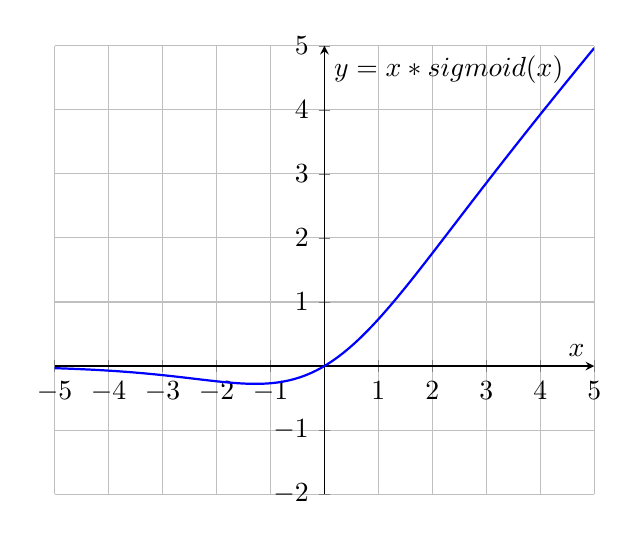
\begin{tikzpicture}
        \begin{axis}[
            xlabel=$x$,
            ylabel={$y = x*sigmoid(x)$},
            axis lines=middle,
            xmin=-5, xmax=5,
            ymin=-2, ymax=5,
            xtick={-5,-4,...,5},
            ytick={-2,-1,...,5},
            grid=both,
            domain=-5:5,
            samples=100,
            smooth,
        ]
        
        \addplot[blue,thick] {x * (1 / (1 + exp(-x)))};
        \end{axis}
    \end{tikzpicture}
    \caption{Swish Graph}
\end{figure}

\subsection{Git}
\lipsum[2][1]


\section{Project Management}

\subsection{Methodology}
\lipsum[2][1]

\subsection{Timeline And Milestones}
\lipsum[2][1]


\section{The Simulation Environment}
\lipsum[2][1]

\subsection{Roads}
\lipsum[2][1]

\subsection{Pathing}
\lipsum[2][1]

\subsection{The Car Control System}
\lipsum[2][1]

\subsection{Environmental Cars}
\lipsum[2][1]

\subsubsection{Car Functionality}
\lipsum[2][1]

\subsubsection{Logical Implementation}
\lipsum[2][1]

\subsubsection{Traffic Light Interaction}
\lipsum[2][1]

\subsection{Traffic Light System}
\lipsum[2][1]

\subsubsection{Target Types}
\lipsum[2][1]

\subsubsection{Logical Implementation}
\lipsum[2][1]

\subsubsection{Smart Traffic}
\lipsum[2][1]


\section{The Agent}
\lipsum[2][1]

\subsection{Introduction To The Agent}
\lipsum[2][1]

\subsection{Proximal Policy Optimisation}
\lipsum[2][1]

\subsection{Controls And Action Space}
\lipsum[2][1]

\subsection{ML-Agents Interaction}
\lipsum[2][1]

\subsection{Deep Neural Network Architecture}
\lipsum[2][1]

\subsubsection{Configuration}
\lipsum[2][1]

\subsubsection{Observations and Outputs}
\lipsum[2][1]

\subsubsection{Hyper-parameters}
\lipsum[2][1]


\section{Reward Systems}
\lipsum[2][1]

\subsection{Weighted Sum}
\lipsum[2][1]

\subsection{Positive Weighted Sum}
\lipsum[2][1]

\subsection{Normalised Rewards}
\lipsum[2][1]

\subsection{Curriculum Learning}
\lipsum[2][1]

\subsubsection{Corner-Slowing}
\lipsum[2][1]

\subsubsection{Lane-Centering}
\lipsum[2][1]

\subsubsection{Environmental Cars And Traffic Lights}
\lipsum[2][1]

\subsubsection{Traffic Lights}
\lipsum[2][1]

\subsubsection{Environmental Cars}
\lipsum[2][1]


\section{Results}
\lipsum[2][1]

\subsection{Evaluation Metrics}
\lipsum[2][1]

\subsection{Reward System Analysis}
\lipsum[2][1]

\subsection{Imitation Learning}
\begin{itemize}
    \item Graph for difference
    \item Reasons why non-imitation is better
    \item Using non-imitation for rest
\end{itemize}

\subsection{Curriculum Learning}
\lipsum[2][1]

\subsection{Final Reward System}
\lipsum[2][1]


\section{Conclusion}
\lipsum[2][1]

\subsection{Main Conclusions}
\lipsum[2][1]

\subsection{Limitations}
\lipsum[2][1]

\subsection{Achievement Discussion}
\lipsum[2][1]


\section{Evaluation}

\subsection{Project Management}
\lipsum[2][1]

\subsubsection{Objectives fulfilment}
\begin{itemize}
\item \textbf{Develop a Realistic Simulation Environment:} Create a Unity-based simulation environment that abstracts real-world driving scenarios, focusing on essential features while omitting minor details.

\item \textbf{Design and Implement Learning Agents:} Develop reinforcement learning agents for the cars, ensuring they can navigate the simulation environment effectively and adapt to changing conditions.

\item \textbf{Conduct In-Depth Research:} Carry out comprehensive research on AI-driven cars, traffic dynamics, and human behaviour to inform the development of the simulation and learning agents.

\item \textbf{Training and Performance Analysis:} Train the AI agents and conduct rigorous performance analysis on the relevant features such as safety, speed, efficiency, and other metrics.

\item \textbf{Varied Situations:} Provide a series of different situations for learning (e.g., traffic lights, cross junctions, t-junctions, pedestrians) to challenge the AI cars to learn more general and applicable behaviours.

\item \textbf{Adapt Agent Based On Feedback:} Tweak and adjust the learning agent rewards depending on its results to better improve its learning capability.

\end{itemize}

\subsubsection{Progress Evaluation}

\subsection{Problems and Oversights}
\lipsum[2][1]

\subsection{Future Outlook}
\lipsum[2][1]



\newpage

\bibliography{sources}
\bibliographystyle{ieeetr} 

\end{document}
